\section*{پاسخ:}

\begin{enumerate}[label=\alph*)]

\item 
\begin{itemize}
    \item \lr{CWR (Congestion Window Reduced)}: زمانی استفاده می‌شود که فرستنده پیامی مبنی بر وقوع ازدحام شبکه (\lr{ECN}) دریافت کرده و نرخ ارسال خود را کاهش داده است.
    \item \lr{ECE (ECN Echo)}: برای اعلام وقوع ازدحام شبکه به فرستنده به‌کار می‌رود، در حالتی که قابلیت \lr{ECN} فعال باشد.
    \item \lr{URG (Urgent)}: نشان می‌دهد بخشی از داده‌ها فوری و با اولویت بالا هستند و باید سریع‌تر پردازش شوند. در این حالت فیلد \lr{Urgent Pointer} معتبر است.
    \item \lr{PSH (Push)}: به گیرنده اطلاع می‌دهد داده‌ها را بدون انتظار برای پر شدن بافر، بلافاصله به برنامهٔ بالادست تحویل دهد (مثلاً در ترافیک تعاملی مانند \lr{SSH} یا \lr{Telnet}).
\end{itemize}

\item 
\[
U = \frac{N \times L/R}{RTT + (L/R)} = \frac{5 \times (1000 \times 8 / 10^6)}{0.12 + (1000 \times 8 / 10^6)} = 0.3125
\]

\item 
در \lr{Go-Back-N} چون با هر خطا نیاز به ارسال مجدد تمام پکت‌های بعدی وجود دارد، هزینهٔ ارسال مجدد بسیار بیشتر از \lr{Selective Repeat} است.  
با افزایش نرخ خطا (\(p\))، امید ریاضی تعداد ارسال مجدد زیاد می‌شود و با توجه به رابطه‌ی \(1 - (1-p)^L \approx pL\)، احتمال خطا در طول بسته افزایش می‌یابد.  
در شبکه‌های دارای ازدحام، این ارسال‌های اضافی باعث افزایش \lr{unneeded duplication} و در نتیجه کاهش محسوس \lr{throughput} می‌شود.

\begin{figure}[H]
    \centering
    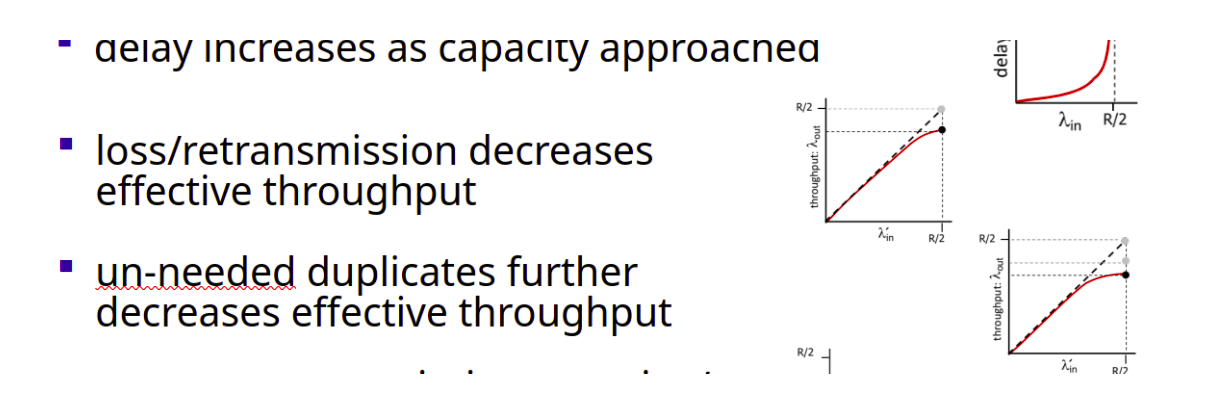
\includegraphics[width=0.95\textwidth]{Solutions/pics/Q2_3_solution.png}
    \caption{تاثیر \lr{Retransmit} و \lr{Un-needed Duplication} بر شبکه}
    \label{fig:small-example}
\end{figure}


\item 
به دلیل محدود بودن فضای شمارهٔ دنباله (فقط چهار مقدار ممکن)، ممکن است گیرنده پکت‌های \lr{retransmit} شده را به‌عنوان پکت جدید در نظر بگیرد.  
برای رفع این مشکل، باید شرط زیر رعایت شود:
\[
\text{Size Window} \leq \frac{\text{Space Sequence}}{2}
\]
در نتیجه اندازهٔ پنجره باید حداکثر برابر با نصف تعداد مقادیر قابل شمارش \lr{sequence number} باشد.

\begin{figure}[H]
    \centering
    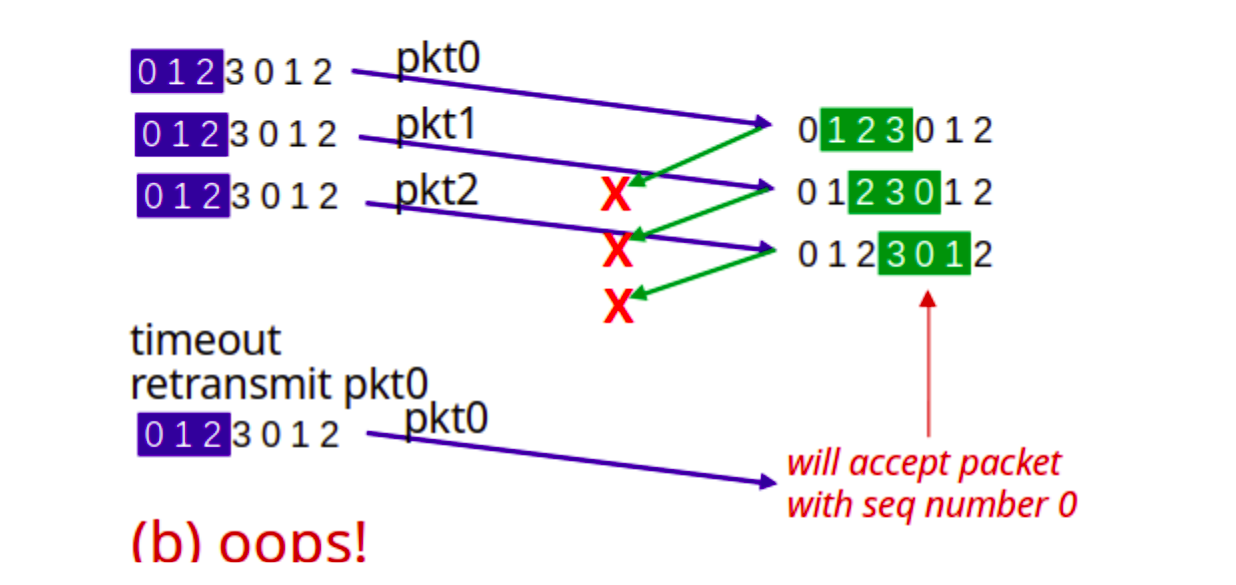
\includegraphics[width=0.95\textwidth]{Solutions/pics/Q2_4_solution.png}
    \caption{}
    \label{fig:small-example}
\end{figure}

\item 
\begin{itemize}
    \item \textbf{FIN:} افزایش \lr{Sequence Number} ضروری است، زیرا در غیر این صورت گیرنده نمی‌تواند تشخیص دهد که \lr{ACK} مربوط به بستهٔ دادهٔ آخر است یا مربوط به پیام پایان ارتباط (\lr{FIN}). این امر می‌تواند منجر به تفسیر اشتباه بسته‌ها شود.
    \item \textbf{SYN:} افزایش \lr{Sequence Number} از نظر فنی ضروری نیست، زیرا در ابتدای ارتباط هیچ داده‌ای وجود ندارد و مقدار \lr{Sequence Number} از ابتدا تصادفی انتخاب می‌شود.  
    اما برای جلوگیری از پیچیدگی و حفظ سازگاری بین دو حالت، در استاندارد \lr{TCP} هر دو پکت \lr{SYN} و \lr{FIN} یک \lr{Sequence Number} مصرف می‌کنند.
\end{itemize}

\end{enumerate}